\documentclass[tikz,border=12pt]{standalone}
\usepackage[T1]{fontenc}
\usepackage{mathpazo}
\usepackage{amsmath,amssymb}
\usetikzlibrary{arrows.meta, positioning, calc}

\definecolor{stblue}{HTML}{7B97AD}
\definecolor{rwgold}{HTML}{B8995E}
\definecolor{sage}{HTML}{7A9A7E}
\definecolor{dkbrown}{HTML}{3D3530}
\definecolor{wmgray}{HTML}{7B7067}
\definecolor{cream}{HTML}{F9F6F0}
\definecolor{border}{HTML}{D4C9B8}
\definecolor{terracotta}{HTML}{C47A6A}
\definecolor{lavender}{HTML}{907EA0}

\begin{document}
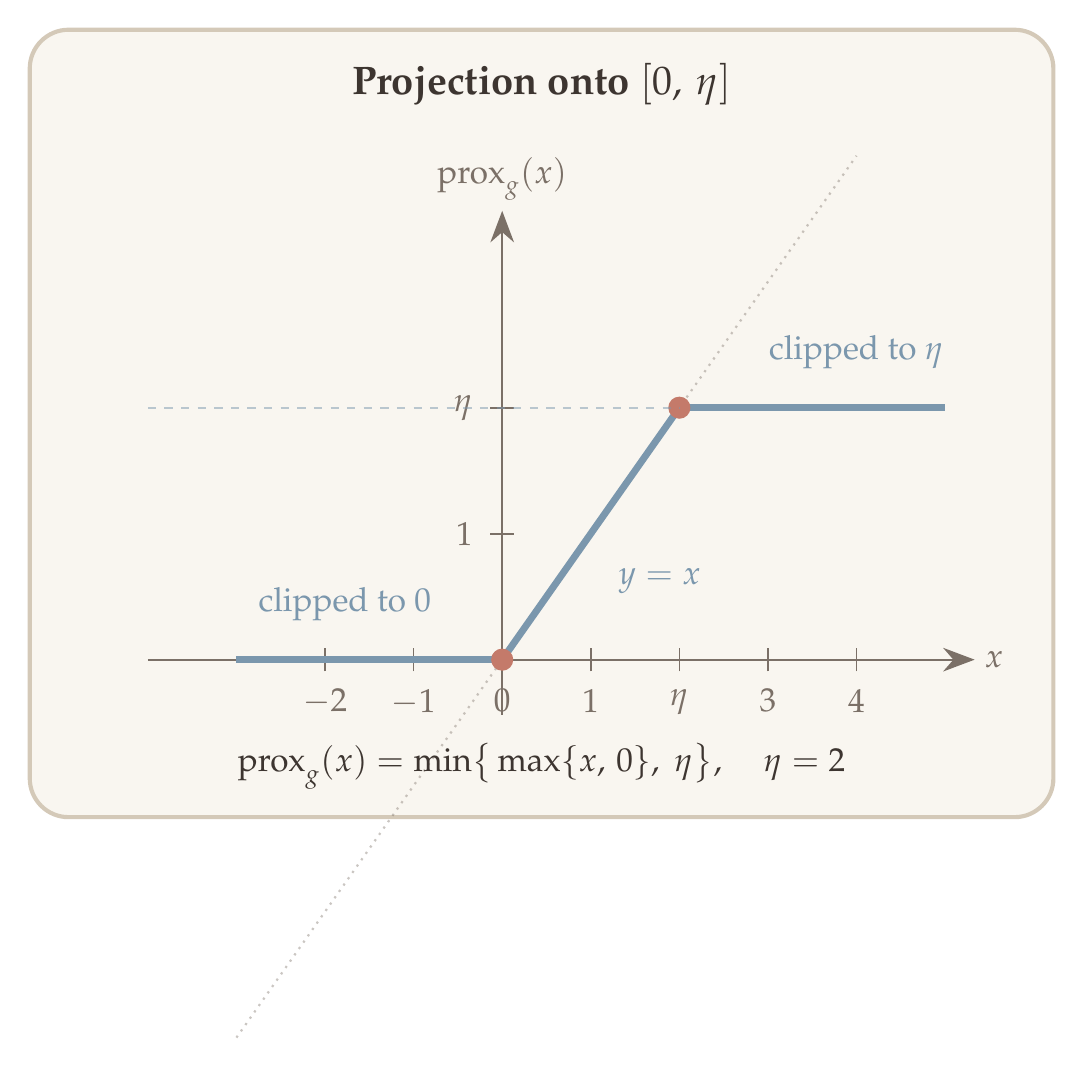
\begin{tikzpicture}[>={Stealth[length=4mm, width=3mm]}]

% Background
\fill[cream, rounded corners=14pt] (-0.5,-0.5) rectangle (12.5,9.5);
\draw[border, line width=1.5pt, rounded corners=14pt] (-0.5,-0.5) rectangle (12.5,9.5);

% Title
\node[text=dkbrown, font=\Large\bfseries] at (6,8.8)
  {Projection onto $[0,\, \eta]$};

% Coordinate mapping:
% x-range: -3 to 5, center at canvas x=5.5 (origin at canvas 5.5)
% y-range: -0.5 to 3, anchor at canvas y=1.5
% x-scale: 1.125, y-scale: 1.6

% Axes
\draw[wmgray, line width=0.8pt, ->] (1.0,1.5) -- (11.5,1.5)
  node[right, font=\large, text=wmgray] {$x$};
\draw[wmgray, line width=0.8pt, ->] (5.5,0.8) -- (5.5,7.2)
  node[above, font=\large, text=wmgray] {$\operatorname{prox}_g(x)$};

% x -> 5.5 + x*1.125
% y -> 1.5 + y*1.6

% Tick marks x-axis
\draw[wmgray, line width=0.6pt] (5.5,1.35) -- (5.5,1.65);
\node[text=wmgray, font=\large, below] at (5.5,1.25) {$0$};

% eta=2 -> canvas x = 5.5 + 2*1.125 = 7.75
\draw[wmgray, line width=0.6pt] (7.75,1.35) -- (7.75,1.65);
\node[text=wmgray, font=\large, below] at (7.75,1.25) {$\eta$};

\draw[wmgray, line width=0.6pt] (4.375,1.35) -- (4.375,1.65);
\node[text=wmgray, font=\large, below] at (4.375,1.25) {$-1$};
\draw[wmgray, line width=0.6pt] (3.25,1.35) -- (3.25,1.65);
\node[text=wmgray, font=\large, below] at (3.25,1.25) {$-2$};
\draw[wmgray, line width=0.6pt] (6.625,1.35) -- (6.625,1.65);
\node[text=wmgray, font=\large, below] at (6.625,1.25) {$1$};
\draw[wmgray, line width=0.6pt] (8.875,1.35) -- (8.875,1.65);
\node[text=wmgray, font=\large, below] at (8.875,1.25) {$3$};
\draw[wmgray, line width=0.6pt] (10.0,1.35) -- (10.0,1.65);
\node[text=wmgray, font=\large, below] at (10.0,1.25) {$4$};

% Y-axis ticks
% eta=2 -> canvas y = 1.5 + 2*1.6 = 4.7
\draw[wmgray, line width=0.6pt] (5.35,4.7) -- (5.65,4.7);
\node[text=wmgray, font=\large, left] at (5.25,4.7) {$\eta$};
\draw[wmgray, line width=0.6pt] (5.35,3.1) -- (5.65,3.1);
\node[text=wmgray, font=\large, left] at (5.25,3.1) {$1$};

% Identity line (dotted reference)
\draw[wmgray, line width=0.8pt, dotted, opacity=0.4]
  (2.125, {1.5 + (-3)*1.6}) -- (10.0, {1.5 + 4*1.6});

% Projection function: min(max(x, 0), eta) with eta=2
% Three pieces:
% 1) x <= 0: y = 0 -> from x=-3 to x=0
%    canvas: (2.125, 1.5) to (5.5, 1.5)
\draw[stblue, line width=2.5pt] (2.125, 1.5) -- (5.5, 1.5);

% 2) 0 <= x <= 2: y = x -> from x=0 to x=2
%    canvas: (5.5, 1.5) to (7.75, 4.7)
\draw[stblue, line width=2.5pt] (5.5, 1.5) -- (7.75, 4.7);

% 3) x >= 2: y = 2 -> from x=2 to x=5
%    canvas: (7.75, 4.7) to (11.125, 4.7)
\draw[stblue, line width=2.5pt] (7.75, 4.7) -- (11.125, 4.7);

% Breakpoint markers
\fill[terracotta] (5.5,1.5) circle (4pt);
\fill[terracotta] (7.75,4.7) circle (4pt);

% Dashed lines showing the clipping levels
\draw[stblue, line width=0.8pt, dashed, opacity=0.5] (1.0, 4.7) -- (7.75, 4.7);

% Annotations
\node[text=stblue, font=\large] at (3.5, 2.2) {clipped to $0$};
\node[text=stblue, font=\large] at (10.0, 5.4) {clipped to $\eta$};
\node[text=stblue, font=\large] at (7.5, 2.5) {$y = x$};

% Formula
\node[text=dkbrown, font=\large] at (6,0.15)
  {$\operatorname{prox}_g(x) = \min\!\big\{\max\{x,\, 0\},\; \eta\big\}$, \quad $\eta = 2$};

\end{tikzpicture}
\end{document}
